\newpage
\subsection{The contact editor}
\label{sec:contacteditor}
The contact editor is used to configure the electrical contacts.  Which layers act as contacts is configured in the layer editor see section \ref{sec:layereditor}.  The contact editor has the following fields:

\begin{figure}[H]
\centering
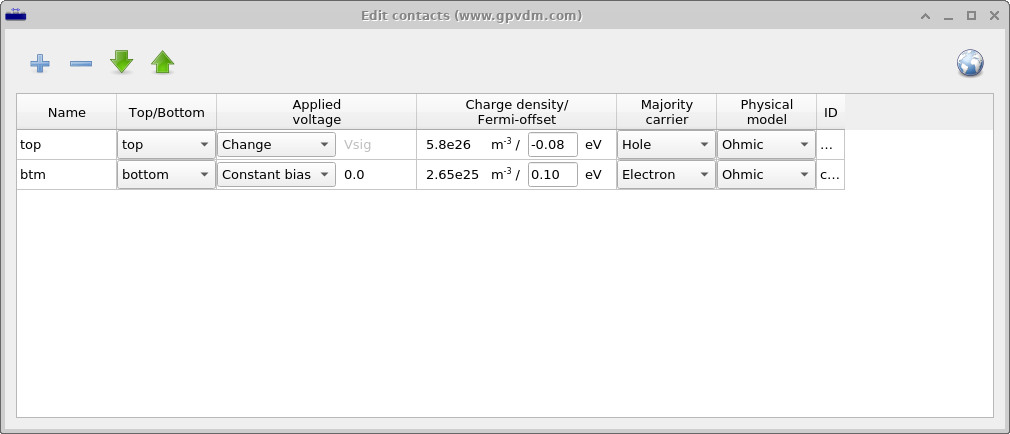
\includegraphics[width=0.5\textwidth,height=0.3\textwidth]{./images/running/contact_editor.png}
\caption{The contact editor}
\label{fig:contacteditor}
\end{figure}

\begin{itemize}
  \item Name: The name of the contact, this can be any English word. It has no physical meaning.
  \item Top/Bottom: Sets if the contact is on the top, bottom or in 2D simulation left and right of the device are also valid.
  \item Applied voltage: Sets the applied voltage on the contact. You first have to select what type of applied voltage you want:
		\begin{itemize}
		\item Ground: This will set the contact to zero volts i.e. ground. 0V is always taken as ground.
		\item Constant bias: This will apply a constant bias to a contact.  It can be set to zero, and would then be equivalent to ground.  In OFET simulations the voltage value can be set to bias one contact to a desired constant voltage.
		\item Change: If a contact is set to 'Change' this tells the simulation to apply a changing voltage to this contact. For example if you are performing a JV sweep, the sweep voltage will be applied to this contact.  Similarly if you are doing an IS simulation (TPV, TPC, ToF etc..) the voltage will be applied/measured to this contact.
		\end{itemize}
  \item Charge density: This sets the majority charge density on the contacts. The Fermi-offset is calculated from the charge density. The model does not use Fermi-offset as an input, it uses charge density.
  \item Majority carrier: This sets the majority carrier density to electrons or holes.
  \item Physical model: This selects if you have ohmic contacts or schottky contacts. I recommend using ohmic contacts.

\end{itemize}

\vspace*{\fill}

\fbox{
\parbox{0.9\textwidth}{
\color{blue} Task \addtocounter{question}{1}\thequestion : For a good contact which results in a high efficiency device, the Fermi-offset will be exactly 0 eV or very small. Firstly set the Fermi-offset to zero for both contacts, and run a simulation.  What efficiency cell do you get? Now set the Fermi-offset to $0.3 eV$ what efficiency cell do you now have? Make a note of the charge densities on the contacts which these Fermi-offsets produce. 
}\par
}


